\documentclass[lettersize,journal]{IEEEtran}
\usepackage{amsmath,amsfonts}
\usepackage{algorithmic}
\usepackage{algorithm}
\usepackage{array}
\usepackage[caption=false,font=normalsize,labelfont=sf,textfont=sf]{subfig}
\usepackage{textcomp}
\usepackage{stfloats}
\usepackage{url}
\usepackage{verbatim}
\usepackage{graphicx}
\usepackage{cite}

% added packages from authors
\usepackage{xcolor}
\usepackage{booktabs} % for \midrule in tables
\usepackage{hhline}
\usepackage{bbm}
\usepackage{bm}
\usepackage{makecell}
\usepackage[mode=buildnew]{standalone}
\usepackage{tikz}
\usetikzlibrary{calc,arrows,patterns,intersections}
\usepackage{pgfplots}
\usepackage{xcolor}
\usepgfplotslibrary{fillbetween}

\hyphenation{op-tical net-works semi-conduc-tor IEEE-Xplore}

\begin{document}


\title{A New Paradigm for Energy Intensive Industries: Adapting to Provide Power Flexibility}

\author{Peter A.V. Gade\textsuperscript{*}\textsuperscript{\textdagger}, Trygve Skjøtskift\textsuperscript{\textdagger}, Henrik W. Bindner\textsuperscript{*}, Jalal Kazempour\textsuperscript{*} \\
    \textsuperscript{*}Department of Wind and Energy Systems, Technical University of Denmark, Kgs. Lyngby, Denmark \\
    \textsuperscript{\textdagger}IBM Client Innovation Center, Copenhagen, Denmark
    % <-this % stops a space
    \thanks{Corresponding author. Tel.: +45 24263865. \\ Email addresses: pega@dtu.dk (P.A.V. Gade), Trygve.Skjotskift@ibm.com (T. Skjøtskift), hwbi@dtu.dk (H.W. Bindner), jalal@dtu.dk (J. Kazempour).}% <-this % stops a space
    \thanks{Manuscript received April 19, 2021; revised August 16, 2021.}}

% \footnote{Corresponding author. Tel.: +45 24263865. \\ Email addresses: pega@dtu.dk (P.A.V. Gade), Trygve.Skjotskift@ibm.com (T. Skjøtskift), hwbi@dtu.dk (H.W. Bindner), jalal@dtu.dk (J. Kazempour).}

% The paper headers
\markboth{Journal of \LaTeX\ Class Files,~Vol.~14, No.~8, August~2021}%
{Shell \MakeLowercase{\textit{et al.}}: A Sample Article Using IEEEtran.cls for IEEE Journals}

\IEEEpubid{0000--0000/00\$00.00~\copyright~2021 IEEE}
% Remember, if you use this you must call \IEEEpubidadjcol in the second
% column for its text to clear the IEEEpubid mark.

\maketitle

% \tableofcontents

\begin{abstract}
    It has been well shown how demand-side flexibility can provide services to the power grid through an aggregator with no emissions. However, the aggregator still faces two, mostly unexplored, fundamental problems: 1) how many demand-side assets are needed in order to achieve a synergy effect? And 2) how are payments allocated to individual flexible providers downstream of the aggregator? This paper answers these two questions using simulations of uncertain assets to illustrate the synergy effect, and Shapley values are used as a payment allocation mechanism. As a use case, manual frequency restoration reserves (mFRR) are used as the ancillary service targeted by the aggregator with real prices from 2022.
\end{abstract}

\begin{IEEEkeywords}
    Demand-side flexibility. mFRR. Synergy effect. Shapley values. Payment allocation.
\end{IEEEkeywords}

\tableofcontents

\section{Introduction}\label{sec:Introduction}

Cite: \cite{shafiei2013modeling}

\subsection{Research questions}

\begin{itemize}
    \item How does the synergy effect materialize for a portfolio of uncertain demand-side assets used for mFRR bidding?
    \item How can payments be fairly allocated to flexible providers in an aggregator portfolio used for mFRR bidding?
\end{itemize}

% \IEEEpubidadjcol

\subsection{Literature review}

While many have studied important aspects of demand-side flexibility such as feasibility and controllability. However, an important aspect has been largely overlooked in the literature. That aspect is the synergy effect related to aggregating a portfolio of demand-side assets (freezers, heat pumps, ventilation systems, etc.).

...

\subsection{Our contribution}

We show two results related to the synergy effect of aggregating many individual demand-side assets with uncertain power consumption. The first is purely statistical and related to the estimation of reserve capacity from the aggregated portfolio versus the individual assets. The second result utilizes the synergy effect of individual \textit{groups} of flexibility providers within a portfolio to allocate payments using Shapley values. It provides an interesting way for an aggregator to assess the performance of flexibility providers within its portfolio which can be used to directly allocate payments which also works in an ex-post setting.

\section{Simulation setup}

\subsection{mFRR}

Ancillary services are used to balance the power grid such that production meets demand to keep the frequency at 50 Hz. In Denmark, mFRR is deployed after fast frequency services when a frequency drop occurs, i.e., it is only used for up-regulation. mFRR participants are paid according to their capacity and their up-regulation. Often, they are not required to up-regulate so their capacity payment constitute a passive income. In our setup, we apply a penalty when the capacity does not match actual up-regulation. For a demand-side aggregator, this could be due to improper capacity estimation or unexpected errors when dispatching assets for up-regulation, e.g., violation of temperature thresholds for TCLs.

We use mFRR reserve prices, balancing prices, and spot prices from DK1\footnote{Western Denmark price zone.}, denoted by $\lambda_{h}^{\text{mFRR}}$, $\lambda_{h}^{\text{b}}$, and $\lambda_{h}^{\text{s}}$ respectively. The constant penalty price for not delivering promised capacity is denoted $\lambda^{\text{p}}$.

The aggregator objective function for mFRR bidding can be written:

\begin{align}\label{eq:mFRRObjective}
     & - \underbrace{\sum_{h=1}^{24} \lambda^{s}_{h}P^{\text{Base}}_{h}}_{\textrm{Energy cost}} + \underbrace{\sum_{h=1}^{24}\lambda_{h}^{\text{mFRR}} p^{\text{mFRR}}_{h}}_{\textrm{Reservation payment}}  \notag \\ & \quad \quad + \underbrace{\sum_{h=1}^{24}  \lambda_{h}^{b} p^{b,\uparrow}_{h}}_{\textrm{Activation payment}} - \underbrace{\sum_{h=1}^{24}  \lambda_{h}^{b} p^{b,\downarrow}_{h}}_{\textrm{Rebound cost}} - \underbrace{ \sum_{h=1}^{24}  \lambda^{p}s_{h}}_{\textrm{Penalty cost}}
\end{align}

Here, $p^{\text{mFRR}}_{h}$ is the hourly mFRR capacity of the aggregator portfolio, $p_{h}^{\text{b},\uparrow}$ is the real-time up-regulation, $p_{h}^{\text{b},\downarrow}$ is the rebound, $s_{h}$ is the energy not delivered, and $p_{\text{Base}}$ the normal operational baseline consumption.

To simplify, we ignore the rebound, i.e., $\lambda_{h}^{\text{b}, \downarrow} = 0$ $\forall{h}$. The energy cost is constant and is not affected by mFRR bidding. Thus, only the reserve and activation payments are considered together with the penalty cost. The profit from mFRR bidding is simply then:

\begin{align}\label{eq:mFRR_profit}
     & \underbrace{\sum_{h=1}^{24}\lambda_{h}^{\text{mFRR}} p^{\text{mFRR}}_{h}}_{\textrm{Reservation payment}} + \underbrace{\sum_{h=1}^{24}  \lambda_{h}^{b} p^{b,\uparrow}_{h}}_{\textrm{Activation payment}} - \underbrace{ \sum_{h=1}^{24}  \lambda^{p}s_{h}}_{\textrm{Penalty cost}}
\end{align}

The challenge for the aggregator in (\ref{eq:mFRR_profit}) is therefore two-fold: 1) $p^{\text{mFRR}}_{h}$ must be estimated and 2) $s_{h}$ should be minimized.

In reality, there is also a bidding process for both capacity and up-regulation but it is ignored here for simplicity. Furthermore, as alluded to in Section \ref{sec:Introduction}, we do not consider the control aspect of the portfolio, i.e., the challenge of effectively following the required response within an hour of up-regulation (although there is also a synergy effect here).

\subsection{Demand-side assets}

In (\ref{eq:mFRR_profit}), the power variables showed total power for the whole aggregator portfolio. Each asset, $i$, in the portfolio has its own power consumption, $p_{h, i}$ $\forall{i} \in \mathbb{I}$. Hence:

\begin{subequations}
    \begin{align}
        p^{\text{mFRR}}_{h}        & = \sum_{h=1}^{24} p^{\text{mFRR}}_{h, i}        \\
        p^{\text{b}, \uparrow}_{h} & = \sum_{h=1}^{24} p^{\text{b}, \uparrow}_{h, i} \\
        s_{h}                      & = \sum_{h=1}^{24} s_{h, i}
    \end{align}
\end{subequations}

An asset could be any power consuming asset\footnote{This including batteries in principle, but these are ignored here.} such as a heat pump, freezer, ventilation system, air condition unit, or boiler, etc. The aggregator can also have large assets such as a zinc galvanizing furnace, pool heating, waste-water centrifugation units, etc.

To keep it simple, we consider assets that deviates from their operational baseline consumption in a uniform manner:

\begin{align}\label{eq:uniform}
    p_{h,i} \thinspace [\text{kW}] = \begin{cases}
                                         1 & \text{if} \quad h = h^{\prime} \sim \mathcal{U}(1,24) \\
                                         0 & \text{otherwise}
                                     \end{cases}
\end{align}

An asset in (\ref{eq:uniform}) could for example be a ventilation unit that is turned on randomly for one hour each day. For an aggregator, it is therefore not possible to estimate $p^{\text{mFRR}}_{h, i}$ accurately, but as $|\mathbb{I}|$ increases, the portfolio consumption converges to a predictable uniform consumption for all $h \in \{1 \hdots 24 \}$ so $p^{\text{mFRR}}_{h}$ becomes predictable.

This fact is readily illustrated in Figure \ref{fig:assets} where a single asset consumes randomly, but the portfolio consumption is uniform and predictable.

\begin{figure}[!t]
    \centering
    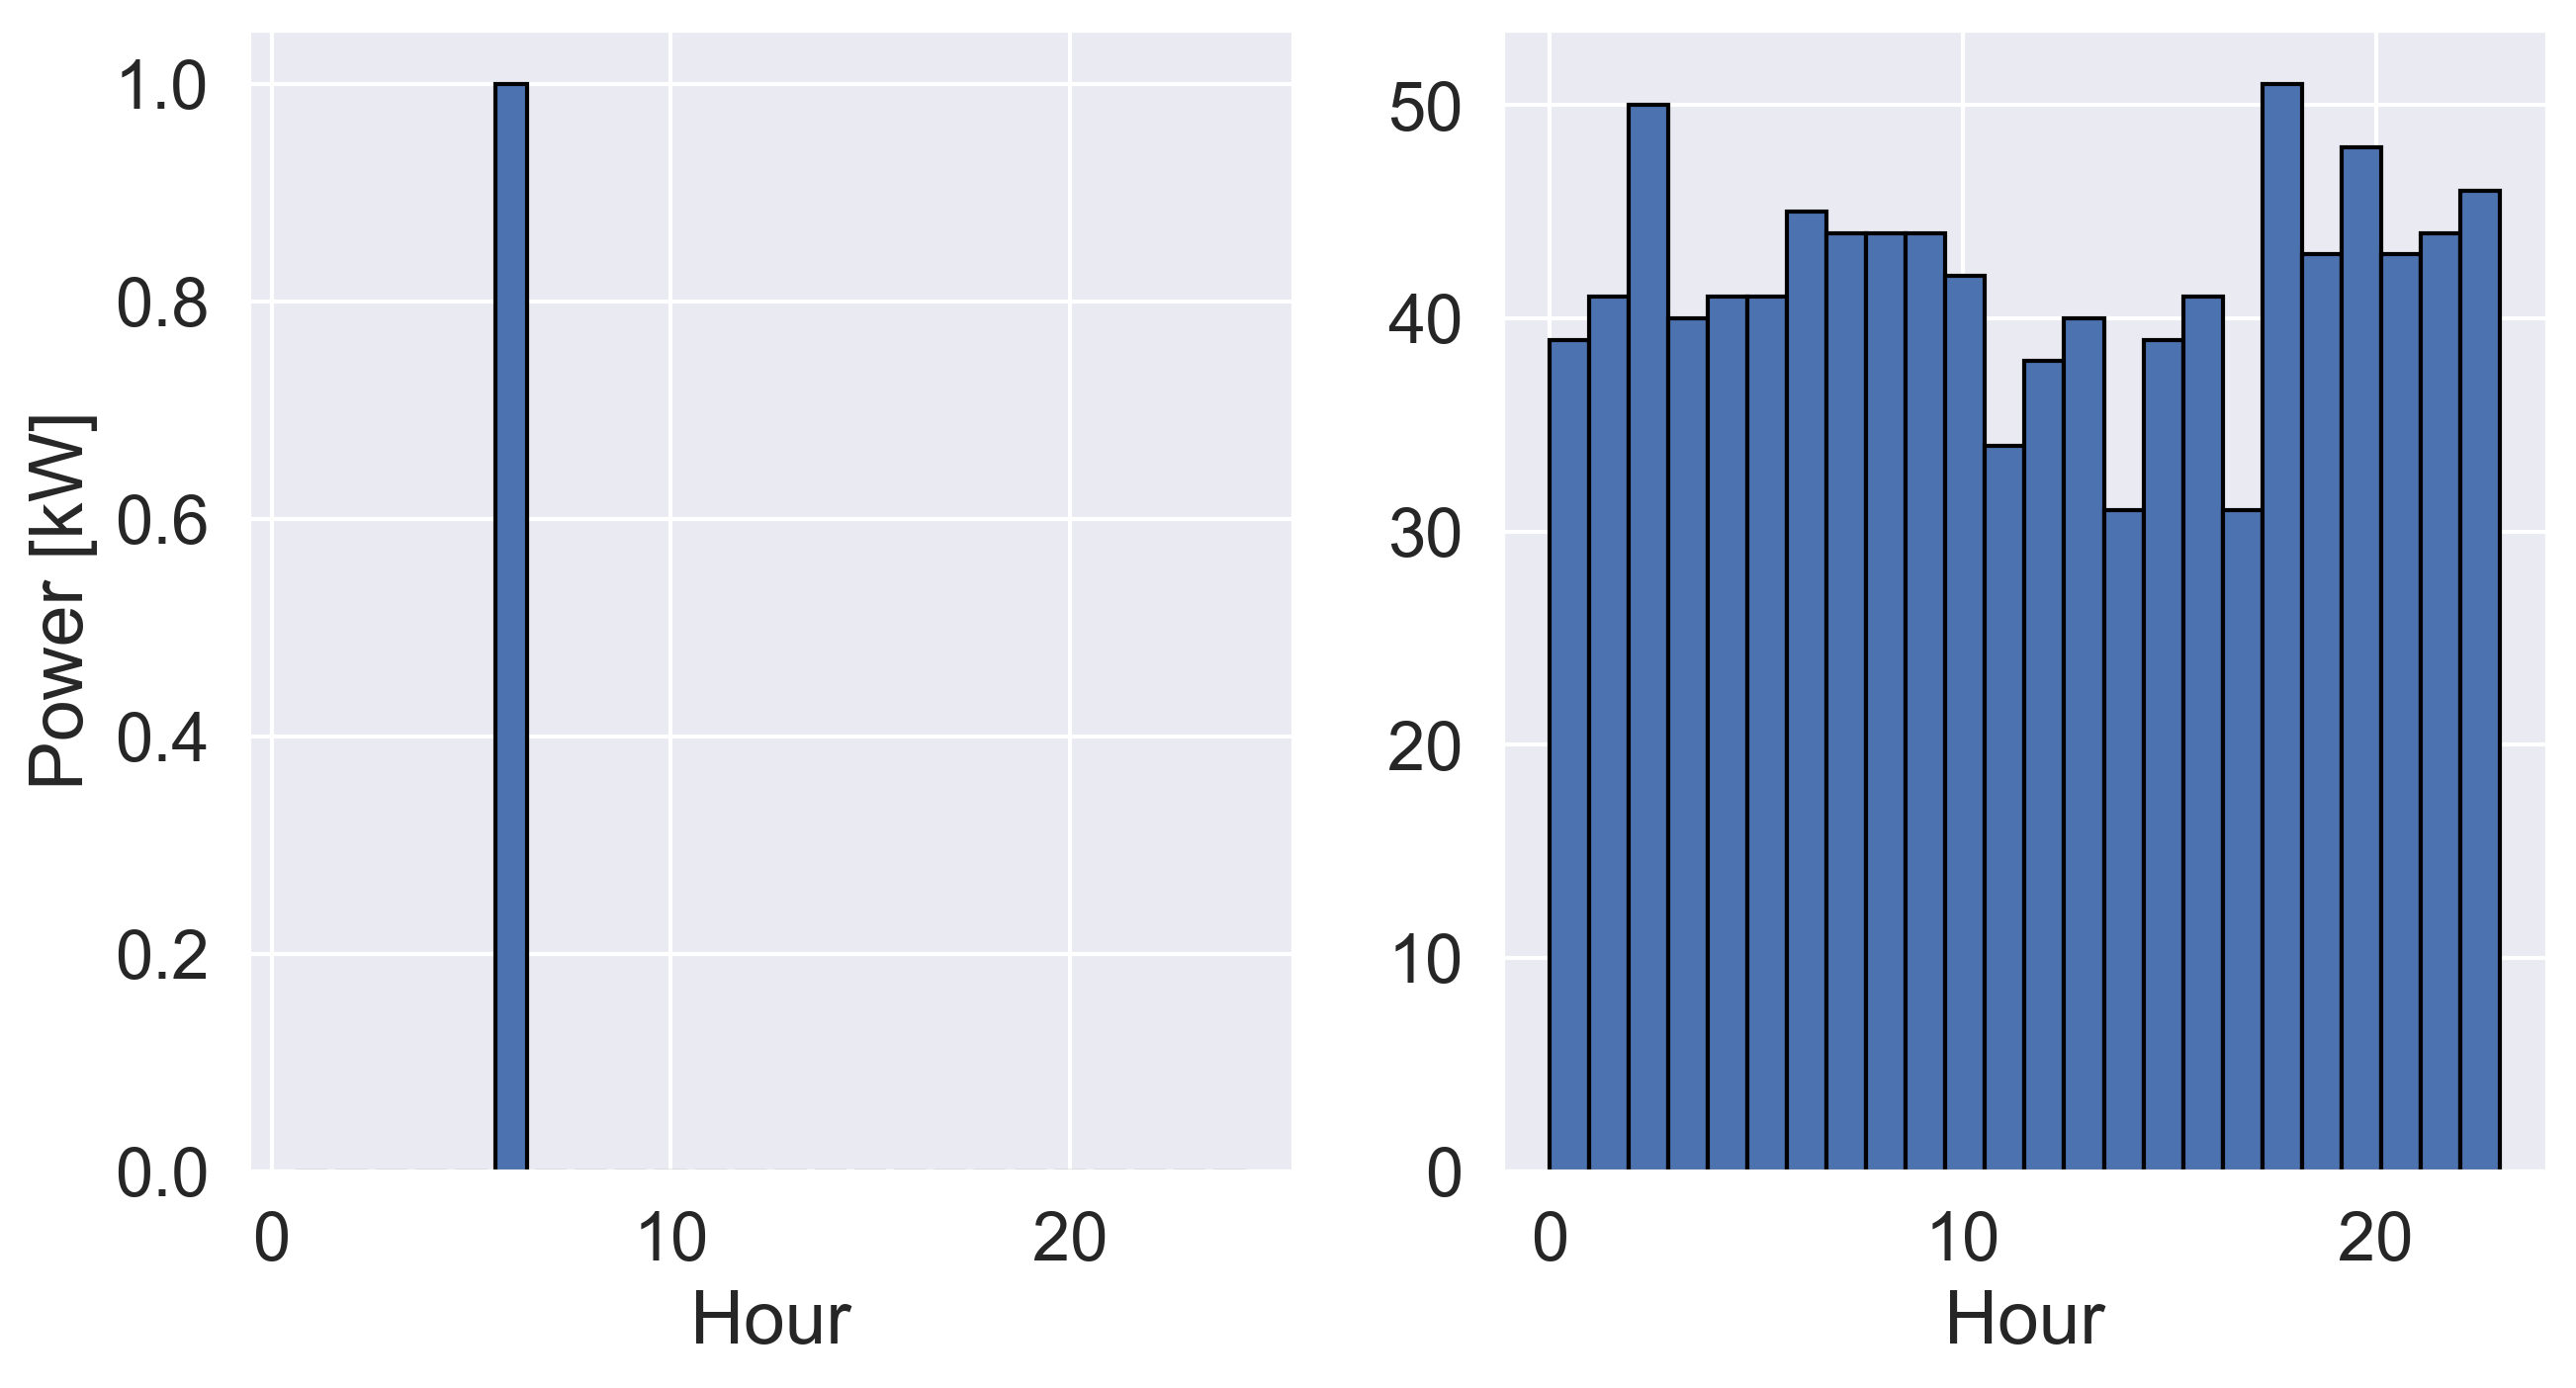
\includegraphics[width=\columnwidth]{figures/assets.png}
    \caption{Simulation of power consumption of assets using (\ref{eq:uniform}). \textbf{Left}: single asset. \textbf{Right}: portfolio of 1000 assets.}
    \label{fig:assets}
\end{figure}


This is of course a stylized example as most assets have some degree of predictability, but it is sufficient to show a very relevant problem for aggregators of small-scale, uncertain demand-side assets: in the beginning, the aggregator cannot estimate the reserve capacity of the portfolio, but as the number of assets increases, it becomes much easier.

With revenue being defined as in (\ref{eq:mFRR_profit}), the synergy effect of the portfolio is then:

\begin{align}\label{eq:synergy_effect}
    \text{Synergy effect [\%]} = \frac{ \text{Portfolio revenue} }{ \sum_{i \in \mathbb{I}} \text{Asset \textit{i} revenue} }
\end{align}


\subsection{Shapley as payment mechanism}

Shapley values is a mechanism to allocate contributions in a cooperative game (cite). This idea fits perfectly with the concept of synergy effect in a portfolio of demand-side assets. The context is now slightly different because we consider a downstream problem of the aggregator, i.e., how much each flex provider (with their assets) contributed to the whole portfolio \textit{ex-post} mFRR bidding. Hence, the aggregator has received a pot of money for the whole portfolio (\ref{eq:mFRR_profit}) and faces the problem of distributing it to flexible providers.

To formalize this problem, we let $g \in \mathcal{G} = \{1 \hdots M \}$ denote a flexible provider in the set of all flexible providers with cardinality $M$. The assets belonging to $g$ are denoted $G_{g,i} = \{1 \hdots N_g \}$. The assets are simulated using the logic in (\ref{eq:uniform}).

Now, the Shapley value for flexible provider $g$ is given by (cite):

\begin{align}\label{eq:shap}
    \phi_g & = \frac{1}{M} \sum_{\mathcal{S} \subseteq \mathcal{G}, g \in \mathcal{S}}\left(\begin{array}{c}
                                                                                                    M-1 \\
                                                                                                    |\mathcal{S}|-1
                                                                                                \end{array}\right)^{-1}[v(\mathcal{S})-v(\mathcal{S} \backslash\{i\})]
\end{align}

Here, $v$ is simply the profit in (\ref{eq:mFRR_profit}). Thus, $v(\mathcal{S})$ represents the value of mFRR bidding for the portfolio of flexible providers given by the set $\mathcal{S}$. The value of the grand coalition, i.e., the whole portfolio is given by $v(\mathcal{G}) = \sum_{g \in \mathcal{G}} \phi_{g}$.

The Shapley value  in (\ref{eq:shap}) can be thought of as the average marginal contribution of flexible provider $g$ across all possible portfolios in $\mathcal{G}$. It can only be computed exactly for small $M$ as the number of possible portfolios is equal to $2^{M} - 1$. As $M$ grows, Shapley values can be approximated (cite).

Using Shapley values as payments, the aggregator have a fair method for allocation. If one flexible provider has assets that contribute little with flexibility, it will be reflected in their Shapley value. For example, a flexible provider can simply have relatively small portfolio of assets. More interestingly, a flexible provider can have high-consuming assets that for some reason are not up-regulating when needed (as illustrated in Section \ref{sec:Results}). Using Shapley values, the aggregator can ex-post determine how much such a flexible provider contributes with. Otherwise, that can be difficult to estimate due to the benefit of reserve payment versus risk of not being able to up-regulate.

Furthermore, the Shapley value has desirable economic properties such as individual rationality (see Section \ref{sec:Results}) and budget balance.

\section{Results}\label{sec:Results}

\subsection{Synergy effect of assets}

Figure \ref{fig:synergy_effect} shows the simulation of the synergy effect using (\ref{eq:uniform}) and (\ref{eq:synergy_effect}) for up to 1000 assets. Even with assets with such uncertain power consumption, it only takes above 150 of these before the synergy effect flattens. In reality, much fewer assets are then needed to estimate their reserve capacity.

As discussed already, this of course ignores the synergy effect of controlling assets \textit{within} each hour to deliver a proper response. This certainly requires a significant number of assets if all of them are ON/OFF controlled and if they are very heterogenous.

\begin{figure}[!t]
    \centering
    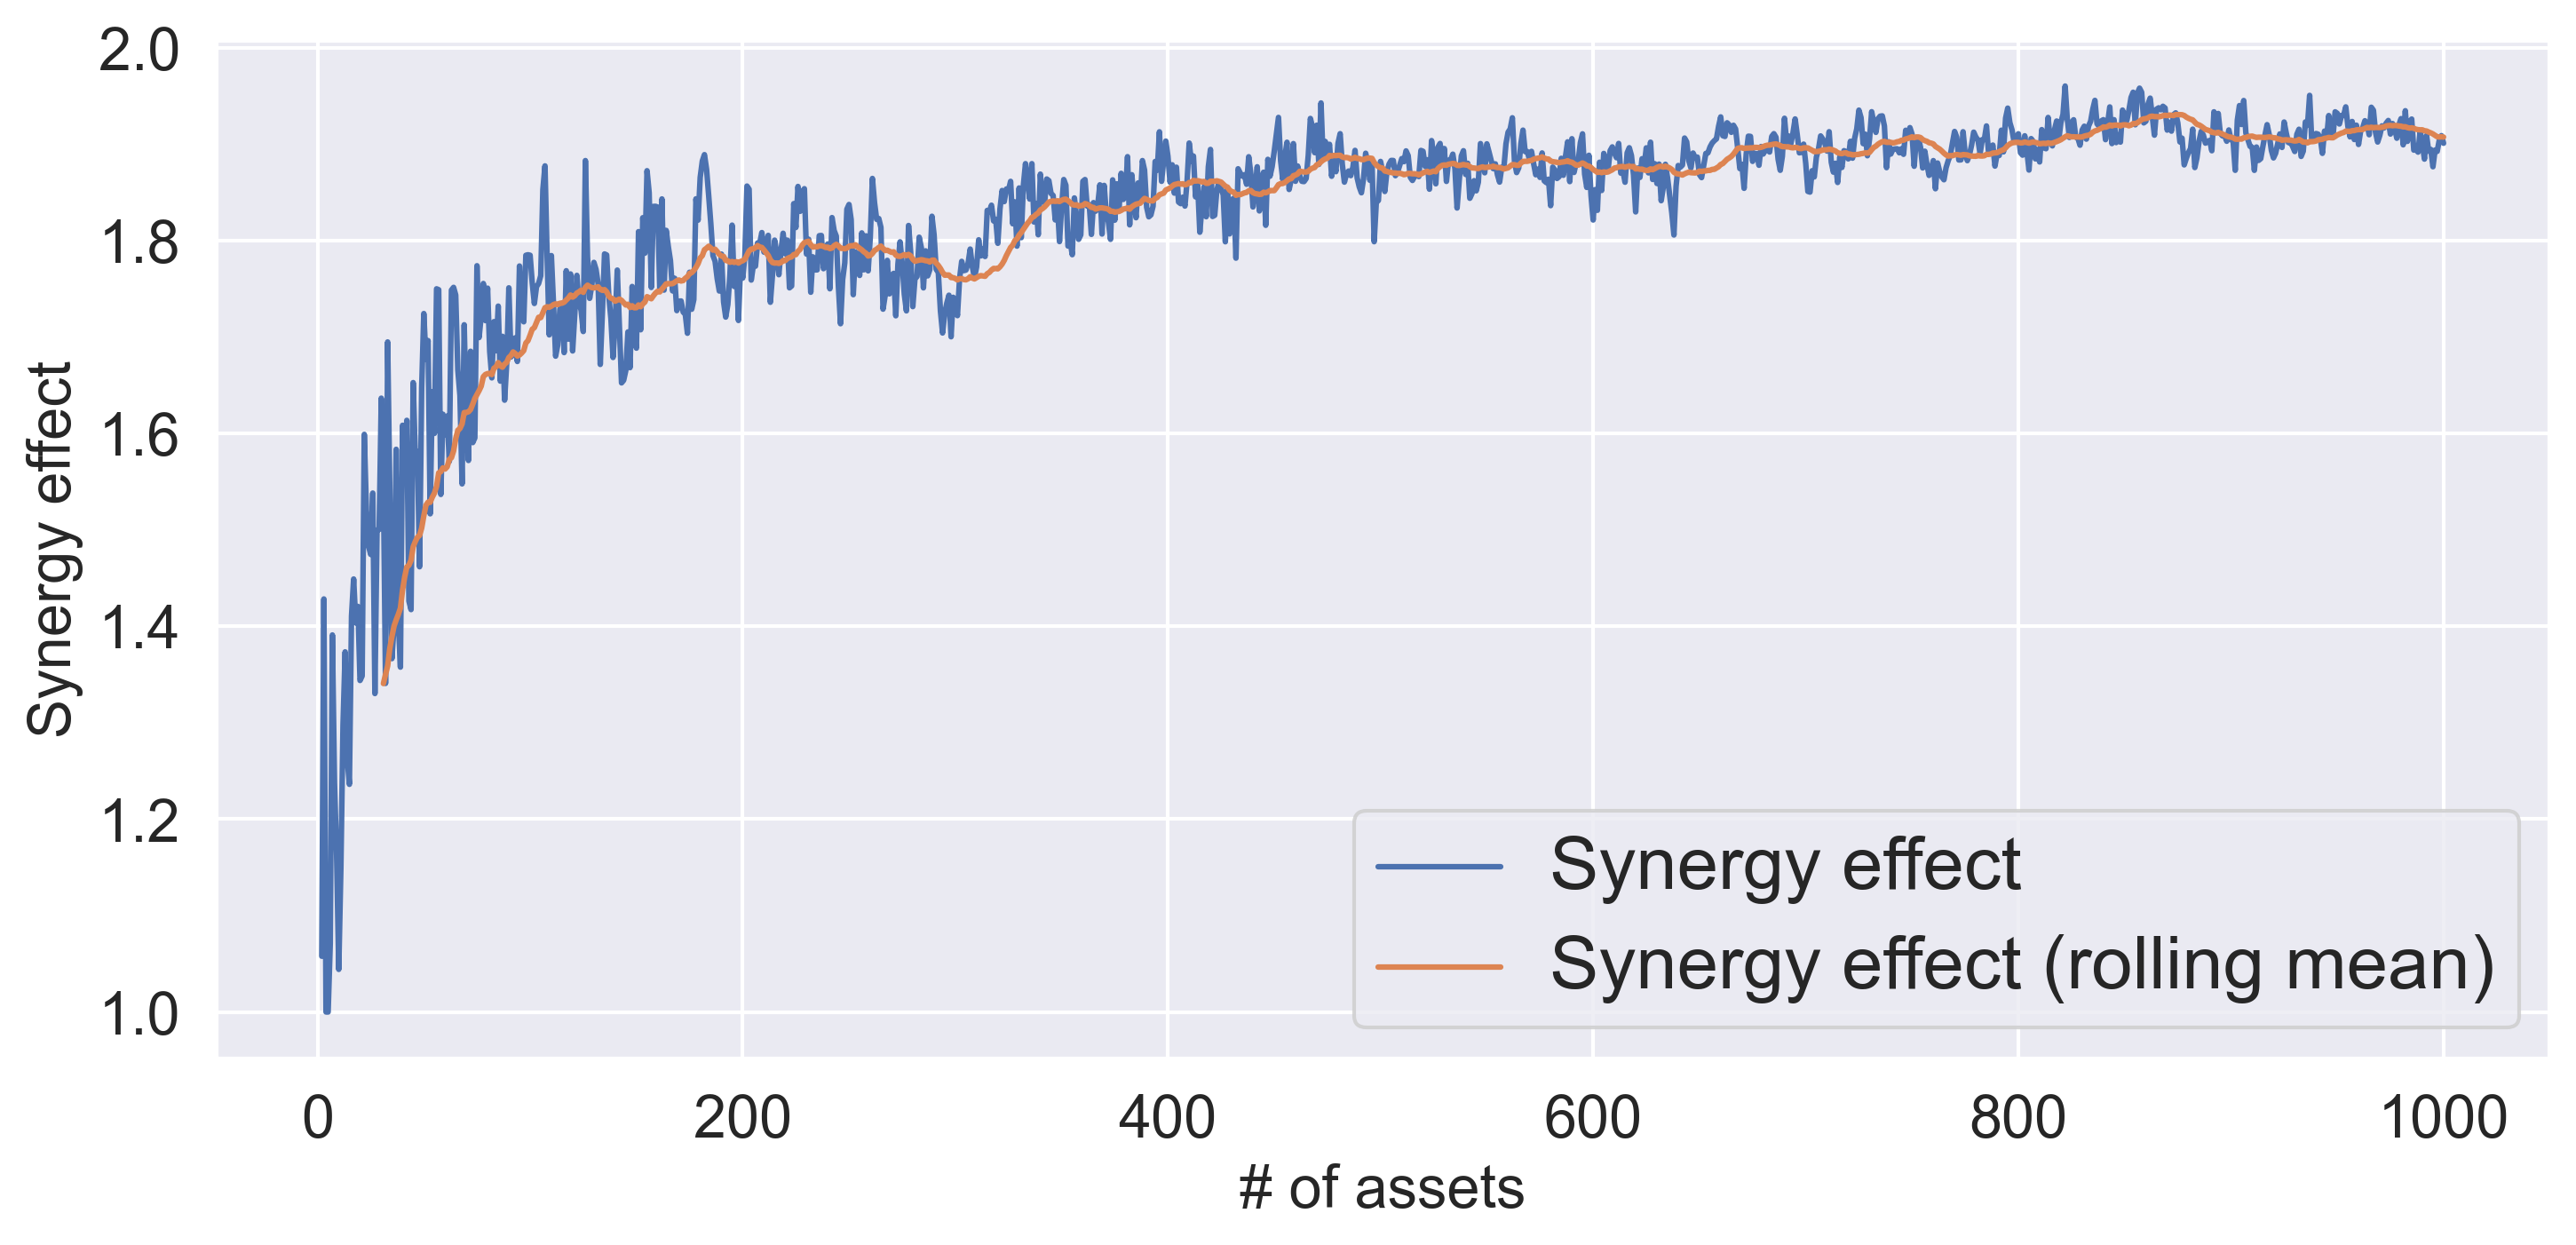
\includegraphics[width=\columnwidth]{figures/synergy_effect.png}
    \caption{Simulation of the impact on the synergy effect by increasing the number of assets. The rolling mean shows the average of the past 40 values.}
    \label{fig:synergy_effect}
\end{figure}

\subsection{Payment allocation}

Figure \ref{fig:shapley_values} shows the Shapley values for a simulation with $M = 6$, and where $g = 1$ has assets that never up-regulates and only contributes with their reserve capacity (which can never be utilized). The simulation is run for increasing values of the penalty parameter, $\lambda^{\text{P}}$. The simulation was run on all price data for 2022.

Interestingly, it shows that the group 1 actually contribute positively to the portfolio when $\lambda^{\text{P}} < ?$. This is simply explained by the price data and how often actual up-regulation is needed (which happens when $\lambda^{\text{B}} > \lambda^{\text{S}}$). If the power grid needed much more up-regulation, the cutoff for $\lambda^{\text{P}}$ would be lower.

The green and orange lines show individual rationality for group $G / \{1\}$: when $\lambda^{\text{P}} < 1.2$ [DKK/kWh], the group is not better off on its own. However, when $\lambda^{\text{P}} > 1.2$ [DKK/kWh], the group is indeed better off on its own because group 1 starts to contribute negatively.

\begin{figure}[!t]
    \centering
    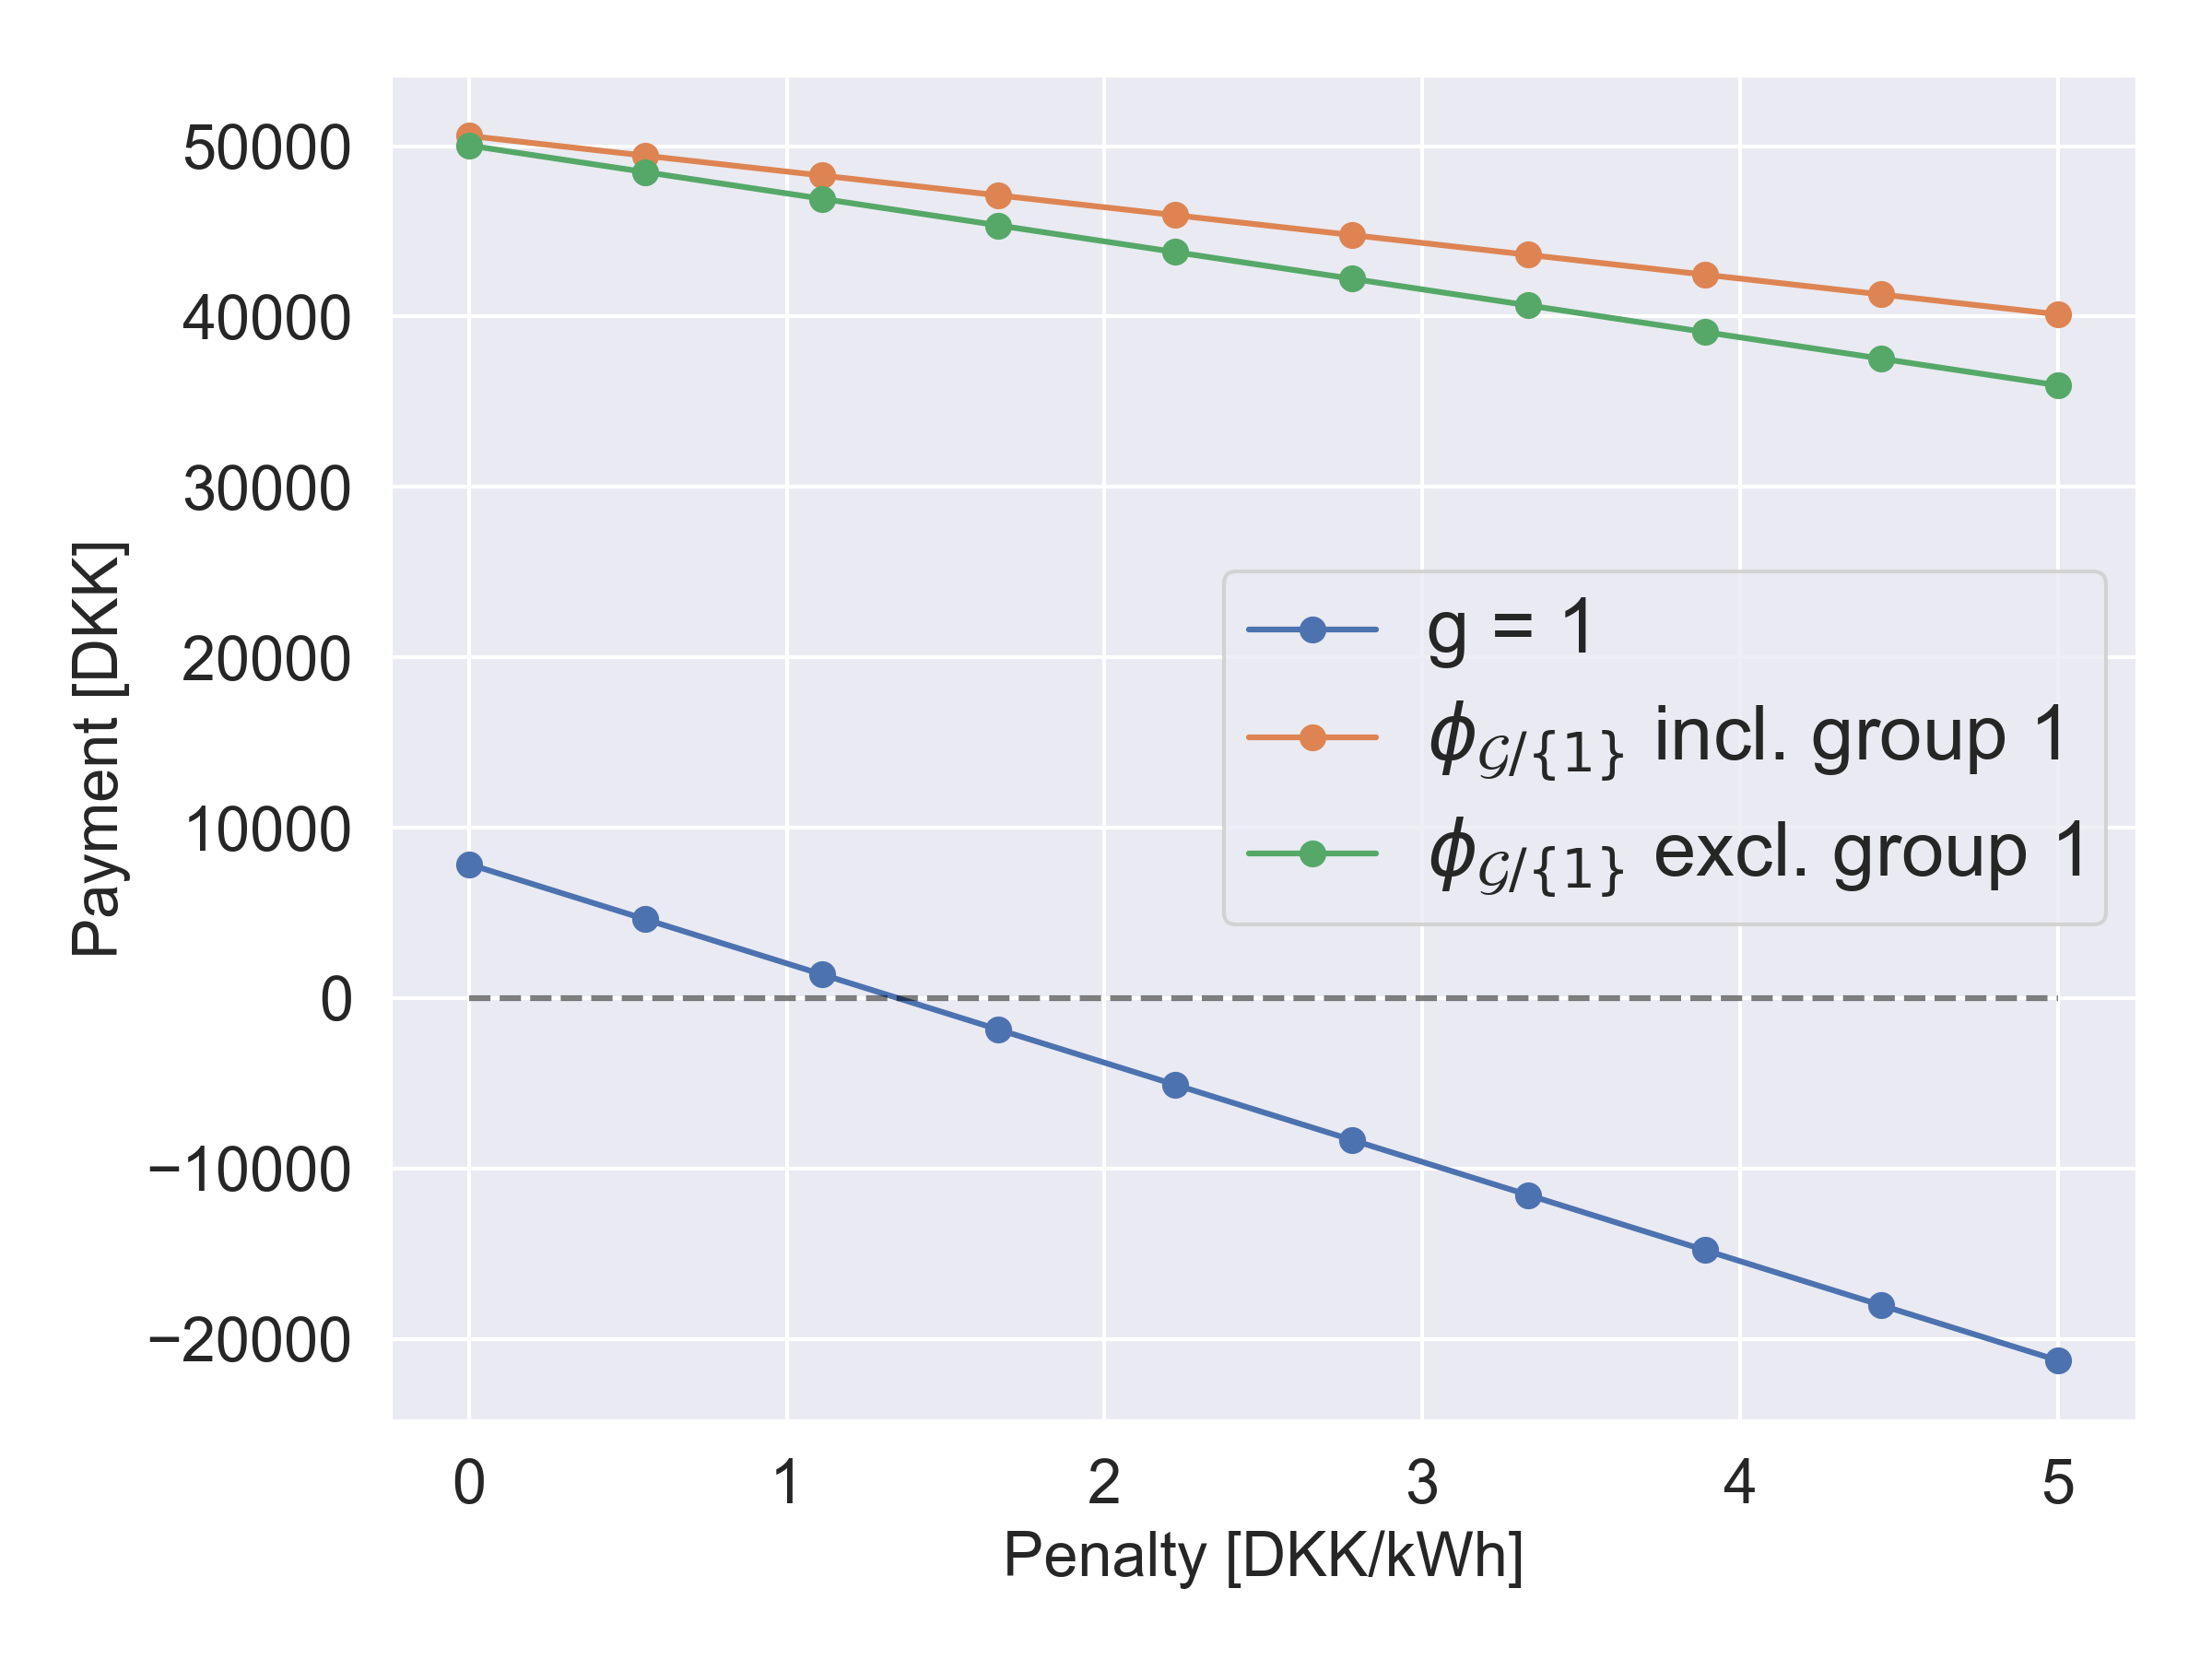
\includegraphics[width=\columnwidth]{figures/shapley_values.png}
    \caption{Simulation of the impact on Shapley values of the penalty price for not delivering promised capacity during up-regulation events. Group 1 has assets with similar power consumption to other groups but no up-regulation.}
    \label{fig:shapley_values}
\end{figure}

\section{Conclusion}



\bibliographystyle{IEEEtran}
% \bibliography{tex/bibliography/Bibliography}
\bibliography{bibliography/Bibliography}


\vfill

\end{document}
